%
%   TEMPLATE
%   コピペ用
%

\documentclass[10pt,b5paper,papersize,dvipdfmx]{jsbook}

\usepackage{vuccaken}
\usepackage{vuccaken2019}

% スタイルファイルの読み込みや自作マクロは、
% 最終的には vuccaken2019.sty の中に書いてください。
% とりあえずはここに書いてもらって構いません。


\begin{document} % - - - - - - - 以下本文 - - - - - - - - - -

\mokuji{2} % 目次出力

% - - - - - - - - - - - - - - - - - - - - - - - - %
\kaishititle%
  {\LaTeX テンプレート(会誌原稿用)}% title
  {物理科学科1回生}% 所属
  {ふじき}% name
% - - - - - - - - - - - - - - - - - - - - - - - - %

%
\section*{はじめに}
今年度から物理科学研究会に入部した物理科1回生の藤木です。\par
今回の会誌では自分は宇宙についてホーキング博士の考えを紹介しながら書いていこうと思っています。

%
\section{第1章 }
はじめにこのファイルのソースを自分のtexファイルにコピペしてください。\par
figureのパスには注意してください。


\clearpage
%
\subsection{figure環境}

\begin{figure}[htbp]
  \centering
  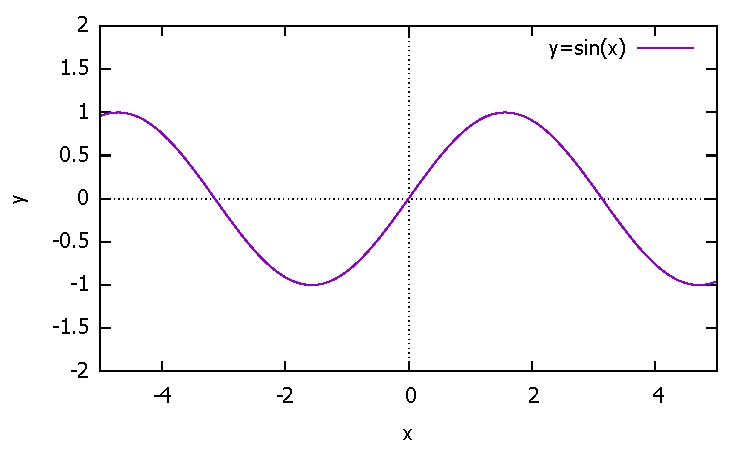
\includegraphics[width=10cm]{temp/fig-sin.pdf}
  \caption{$y=\sin x$のグラフ。gnuplotで作成した。}
  \label{fig:sin}
\end{figure}

図\ref{fig:sin}はイケメンです。

%
\subsection{table環境}

\begin{table}[htbp]
  \centering
  \caption{やさいの表}
  \label{tbl:vegetable}
  \begin{tabular}{r|ccc} \hline
      No. & やさい & いろ & 印象 \\ \hline
      1 & トマト & あかいろ & くさい \\
      2 & キャベツ & みどり & 無味乾燥 \\
      3 & かぼちゃ & きいろ & かたい \\
      4 & にんじん & おれんじ & ゴミ \\ \hline
  \end{tabular}
\end{table}

表\ref{tbl:vegetable}は僕の主観です。


%% 参考文献
\begin{thebibliography}{99}
  \item 著者, 本やページの名前, (URL), 出版社, 出版年.
  \item (複数ある場合は追加)
  \item @vuccaken, 物科研HP, \url{https://vuccaken.github.io}, 2019.
  % \bibitem{キー1} 著者, 本やページの名前, (URL), 出版社, 出版年.
\end{thebibliography}


\end{document} % - - - - - - - - - - - - - - - - - - - - -
%
% ファイトだよ!
%